\documentclass{beamer}

\usepackage[american,russian]{babel}

\usefonttheme{serif}

\setbeamertemplate{footline}[frame number]{}
\setbeamertemplate{navigation symbols}{}

\usecolortheme{default}
\setbeamercolor{block title}{bg=lily!20,fg=black}
\setbeamercolor{block body}{bg = blue!10, fg = black}
\setbeamertemplate{itemize item}[square]
\setbeamercolor{itemize item}{fg = cyan}
\setbeamercolor{enumerate item}{fg = cyan}

\usetheme{default}
\usepackage{caption}

%\setbeamercolor{titlelike}{fg=cyan}
%Information to be included in the title page:

\title[About Beamer] %optional
{Оптический пробой сред}

%\subtitle{A short story}

\author[Arthur, Doe] % (optional, for multiple authors)
{A.~Simankovich \and D.~Dedkov }

\institute[VFU] % (optional)
{
	Moscow Institute of Physics and Technology
}

\date[VLC 2023] % (optional)
%{Very Large Conference, April 2021}

%\logo{\includegraphics[height=1cm]{overleaf-logo}}

\begin{document}
	
	\frame{\titlepage}
	
	\begin{frame}
		\frametitle{Аннотация}
		
		TODO: Аннотация
		
		Article studies He-Ne laser and it's basic principle of operation. Laser gain is measured. Feasibility of Malus' law is demonstrated. Mode structure of laser is examined.

	\end{frame}


	\begin{frame}[plain,c]
		
		\begin{center}
			\huge \usebeamercolor[fg]{frametitle} Введение
		\end{center}
	
	\end{frame}
	
	
	\begin{frame}
		\frametitle{Статический пробой}

		\begin{figure}
			\includegraphics[width=0.8\linewidth]{res/const_discharge.jpg}
		\end{figure}
		
		\begin{columns}
			\column{0.6\linewidth}
			\begin{figure}
				\includegraphics[width=\linewidth]{res/paschen.jpg}
			\end{figure}

			\column{0.5\linewidth}
			Самый известный и хорошо изученный тип пробоя -- пробой постоянным напряжением. Его поведение в первом приближении описывается кривыми Пашена.
			Заметим, что у кривой существует минимум.
		\end{columns}
		
		
	\end{frame}

	\begin{frame}
		\frametitle{Пробой в переменных полях}
		
		\begin{figure}
			\centering
			\captionsetup{justification=centering}
			\includegraphics[width=0.8\linewidth]{res/microwave_discharge.png}
			\caption*{Зависимость пробойного поля от давления\\ ($f = 992$ МГц, диффузионная длина $0.631$ см)}
		\end{figure}
		
		%TODO: ссылка на Microwave Breakdown in Gases by A. D. MacDONALD
		Под действием переменного поля также возникает пробой. Его минимум для типичных параметров установки расположен в диапазоне давлений, близких к нормальному.
	\end{frame}

	\begin{frame}
		\frametitle{Оптический пробой}
		\begin{figure}
			\centering
			\captionsetup{justification=centering}
			\includegraphics[width=0.6\linewidth]{res/femtosecond_laser_spark.jpg}
			\caption*{Пробой воздуха фемтосекундным лазером}
		\end{figure}
		%TODO: может не стоит вставлять картинку с непонятной радугой?
		В данной работе изучается пробой полем оптического диапазона. Характерные значения поля для пробоя $E \approx 10^6 \div 10^7$ В/см (для постоянного и СВЧ полей $E \approx 3 \cdot 10^4$ В/см). 
		$$ P \approx 30 \text{ МВт}, \quad d = 2 \cdot 10^{-2} \text{ см} $$
		$$ I \approx 10^5 \text{ МВт/см}^2, \quad E \approx 6 \cdot 10^6 \text{ В/см} $$

		%Такие величины полей достижимы только в фокусированном лазерном излучении: при пиковой мощности и диаметре фокуса $2 \cdot 10^{-2}$ см получаем $I \approx 10^5$ МВт/см$^2$ и поле $E = 6 \cdot 10^6$ В/см.
	
	\end{frame}

	\begin{frame}
		\frametitle{Применения лазерного пробоя}
	
		\begin{figure}
			\centering
			\captionsetup{justification=centering}
			\includegraphics[width=0.5\linewidth]{res/libs.jpg}
			\caption*{Лазерно-искровая эмиссионная спектрометрия}
		\end{figure}
			
		Лазерно-искровая эмиссионная спектрометрия является основным прикладным применением лазерного пробоя.
		
		Также явление лазерного пробоя тесно связано с задачами термоядерного синтеза.
		
		Изучение лазерного пробоя позволяет получить важные выводы для квантовой теории.
		
	\end{frame}
	
	\begin{frame}
		\frametitle{Стадии искры}
		\begin{figure}
			\centering
			\captionsetup{justification=centering}
			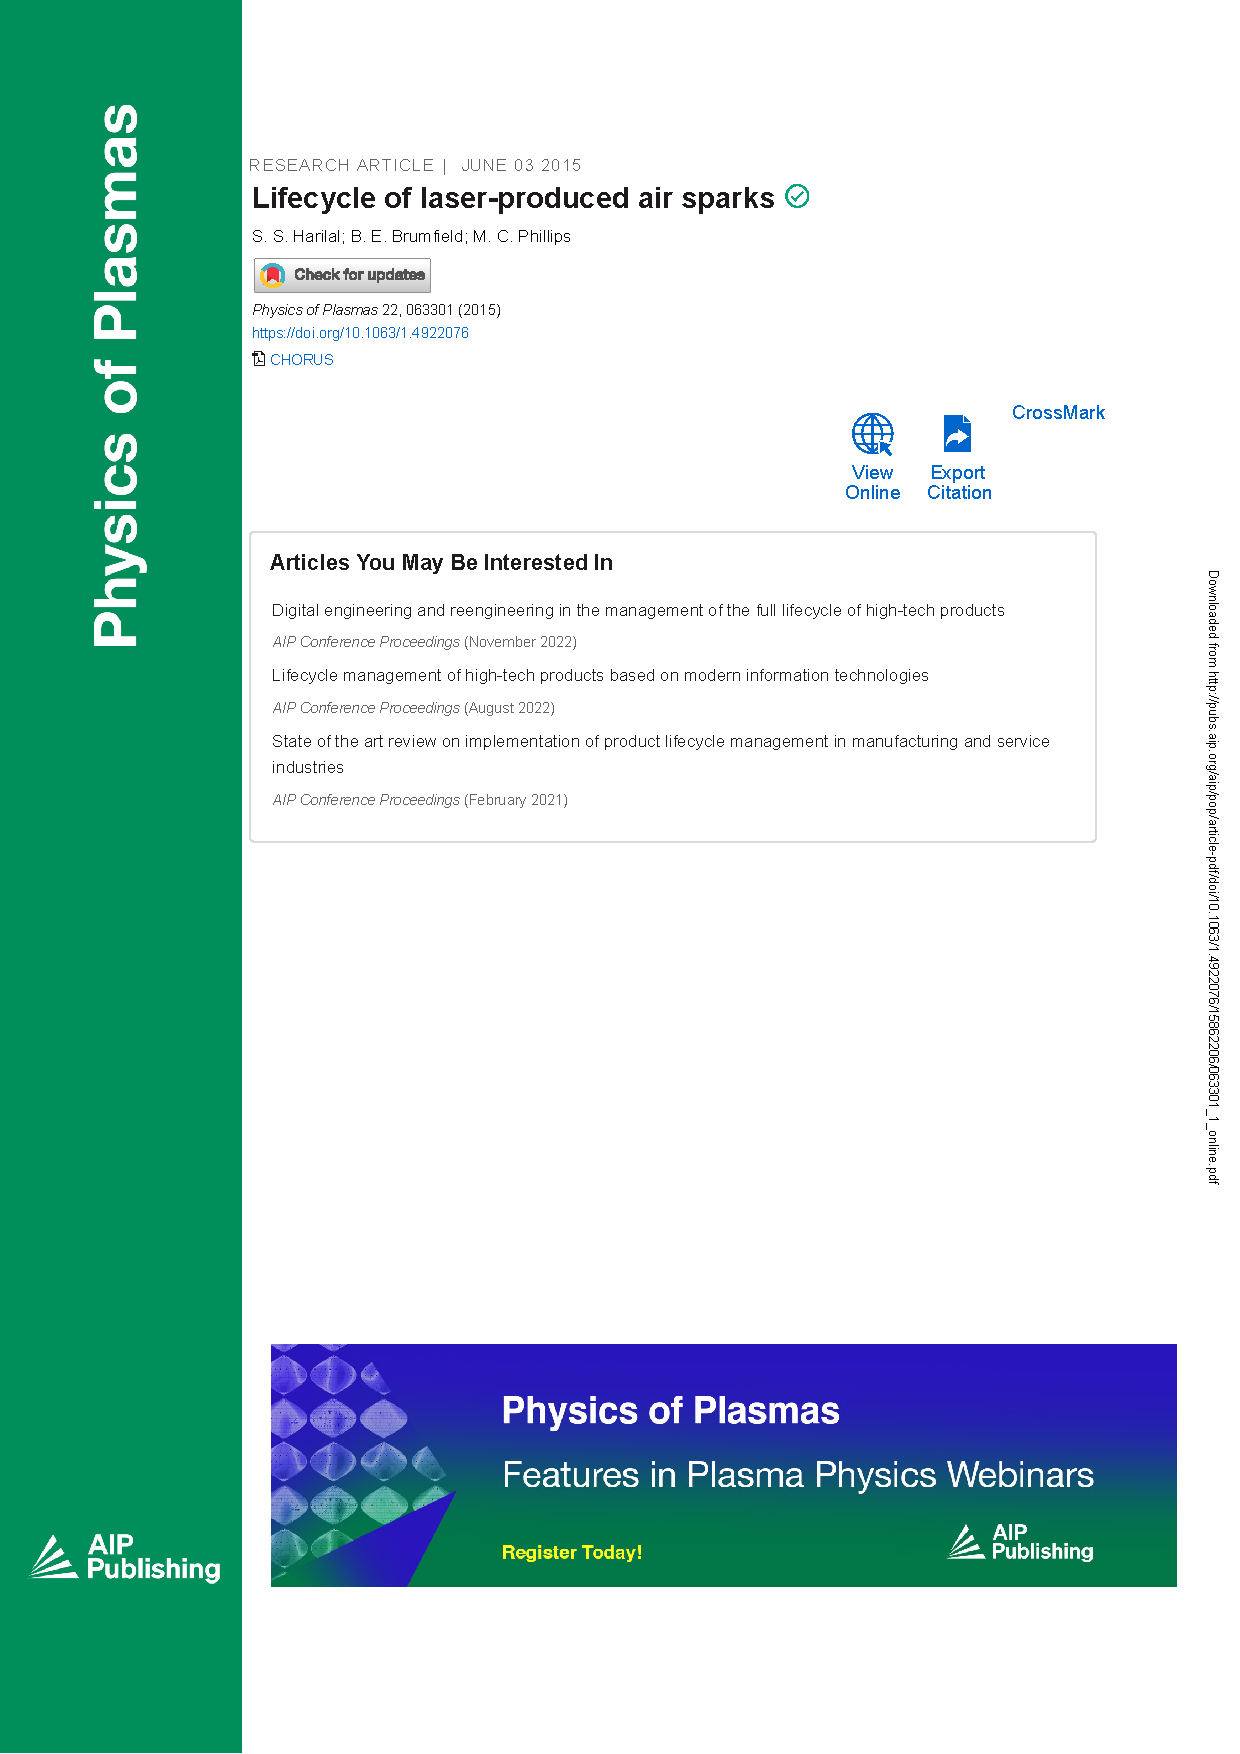
\includegraphics[width=0.8\linewidth]{res/spark_evolution.png}
			\caption*{Эволюция воздушной искры во времени}
		\end{figure}
		\vspace{-5pt}
		Явление лазерной искры можно разделить на три стадии:
		\begin{itemize}
			\item Пробой: ионизация и появление начальной плазмы.
			\item Взаимодействие плазмы с лазерным импульсом, движение плазменного фронта.
			\item Распространение ударной волны, свечение.
		\end{itemize}
		
		
		\begin{columns}
			\column{0.33\linewidth}
			
			\column{0.33\linewidth}
			\column{0.33\linewidth}
		\end{columns}
		TODO: Три стадии искры, Райзер с.9, картинка из наносекундной съемки
	\end{frame}
	
	
	\begin{frame}[plain,c]
		
		\begin{center}
			\huge \usebeamercolor[fg]{frametitle} Theory
		\end{center}
		
	\end{frame}
	
	\begin{frame}
		\frametitle{Два механизма оптического пробоя}
		1.
		Под действием постоянного внешнего электрического поля свободные электроны ускоряются, при столкновении с атомом рассеивая эту энергию в тепло. В осциллирующем поле, при колебании электронов, в среднем энергия электронов при столкновениях тоже переходит в тепло. Таким образом, в области поля средняя скорость электронов увеличивается. Эти электроны набирают достаточную энергию, чтобы ионизировать атомы. Новые электроны добавляются к свободным, увеличивая скорость ионизации. Таким образом формируется электронная лавина.
		
		Для оптического диапазона разумнее использовать квантовую теорию. При столкновениях с атомами электрон поглощает фотоны, приобретая энергию. Этот процесс обратен тормозному испусканию квантов при рассеянии.
		
		2. Вторым механизмом является многоквантовый фотоэффект. Электрон может оторваться от атома вследствие одновременного поглощения сразу нескольких фотонов. Одноквантовый эффект невозможен, так как энергия ионизации ()$I \sim 10\div20$ эВ) на порядок выше энергии фотонов видимого диапазона ($ h\nu = \sim 2$ эВ).
		
		Для газов при атмосферных давлениях и выше характерен первый механизм.
	\end{frame}
	
	\begin{frame}
		\frametitle{Простейшая оценка напряженности поля}
		
		Для вырывания электрона из атома есть два механизма: туннельный эффект (например, в статическом электрическом поле) и многоквантовый фотоэффект.
		
		Ширина потенциального барьера под действием поля $E$ составляет $\Delta \sim \frac{I}{eE}$. Скорость электрона $v \sim \sqrt{I/m}$. Тогда время пролета барьера $\tau \sim \Delta / v \sim \frac{\sqrt{Im}}{eE}$. Туннелирование может происходить если поле остается 'стационарным' во время пролета барьера: $\omega \tau \ll 1$. Для многоквантовости требуется обратное неравенство: $\omega \tau \gg 1$. Для типичных значений лазерного излучения характерно $\omega \tau \gg 1$.
		
	\end{frame}
		
	\begin{frame}
		\frametitle{Простейшая оценка напряженности поля}
		\footnotesize
		Попытаемся оценить пороговое значение поля с помощью теории многоквантового фотоэффекта.
		
		Вероятность многоквантового фотоэффекта $w$ с поглощением $n$ фотонов пропорциональна $n$-ой степени потока квантов $w \sim F$, то есть $w \sim E^{2n}$.
		
		$w \sim \frac{1}{I^n}$ -- чем выше порог ионизации, тем ниже вероятность.
		$w \sim \frac{1}{\omega^n}$ -- чем ниже частота поля, тем больше характерное время изменения поля, за которое электрон может поглотить нужную энергию.
		
		$$ w \sim \left(\frac{E^2}{\omega I}\right)^n$$
		Точный расчет был произведен Л.В.Келдышем с использованием квантовой механики, его результат для фотоэффекта можно аппроксимировать следующей формулой:
		$$ w = B \omega n^{3/2} \left(\frac{\overline{e} \pi e^2}{mc} \frac{\hbar E}{\omega I}\right)^n,$$
		где $\omega$ -- частота поля,
		
		TODO: Райзер, с 15, дописать численную оценку
		
		Получить формулу как-то просто не получается(
	\end{frame}

	
	\begin{frame}
		\frametitle{Нарастание энергии}
		
		TODO: Райзер, с 19-22 (вывод довольно простой)
		
		KEKW: Классическая теория не описывает оптический диапазон: $h\nu >> \varepsilon_{\text{кол}}$.
		
		KEKWKEKW: А нет, описывает: $ h \nu >> \varepsilon_{\text{кол}}$, но $h\nu << \varepsilon$, а это новое условие применения классики (Райзер, с 40, 43)
	\end{frame}
	
	\begin{frame}
		TODO: 6 глава, оттуда вытащить более точное значение порога
	\end{frame}
	
	
	
	
	\begin{frame}
		\frametitle{Elementary processes}
		
%		\begin{columns}[t]
%			\footnotesize
%			
%			\column{0.33\linewidth}
%			\includegraphics[height=3cm]{res/emission_types_1.jpg}
%			$$\left(\frac{dN_0}{dt}\right)_{\text{abs}} = - B_{01} N_0 \rho(\omega)$$
%			Einstein coefficients are the same $B_{01} = B_{10} = B$ 
%
%			\column{0.33\linewidth}
%			\includegraphics[height=3cm]{res/emission_types_2.jpg}
%			$$\left(\frac{dN_0}{dt}\right)_{\text{stim}} = B_{10} N_1 \rho(\omega)$$
%			phase, direction and frequency of emitted and external photons are identical.
%		
%			\column{0.33\linewidth}
%			\includegraphics[height=3cm]{res/emission_types_3.jpg}
%			$$\left(\frac{dN_0}{dt}\right)_{\text{spon}} = - A_{10} N_1$$
%			photons radiate independently in all directions. $\frac{dN_0}{dt}$ \textbf{does not} depend on $\rho(\omega)$.
%		\end{columns}
		
		\vspace{10pt}
		\footnotesize
		Where $\rho(\omega)$ -- spectral energy density of the isotropic radiation field at the frequency of the transition.
	\end{frame}

	\begin{frame}
	\frametitle{Laser Gain}
	
%	\begin{figure}
%		\centering
%		\includegraphics[width=1\linewidth]{res/general_laser_scheme.pdf}
%		\caption{General laser scheme}
%		\label{fig:general_laser_scheme}
%	\end{figure}
	Beer–Lambert–Bouguer law states that intensity of light $I(x)$ changes:
	$$I(x) = I_0 \exp({\gamma x}),$$
	
	where $\gamma$ -- medium gain coefficient. With length $L$ gain per period is called \textbf{laser gain}:
	
	$$G = \exp{(\gamma L)}.$$
	\end{frame}
	
	\begin{frame}[plain,c]
		
		\begin{center}
			\huge \usebeamercolor[fg]{frametitle} Thank you for your attention!
		\end{center}
		
	\end{frame}
	
\end{document}